% Options for packages loaded elsewhere
\PassOptionsToPackage{unicode}{hyperref}
\PassOptionsToPackage{hyphens}{url}
%
\documentclass[
]{book}
\usepackage{amsmath,amssymb}
\usepackage{lmodern}
\usepackage{ifxetex,ifluatex}
\ifnum 0\ifxetex 1\fi\ifluatex 1\fi=0 % if pdftex
  \usepackage[T1]{fontenc}
  \usepackage[utf8]{inputenc}
  \usepackage{textcomp} % provide euro and other symbols
\else % if luatex or xetex
  \usepackage{unicode-math}
  \defaultfontfeatures{Scale=MatchLowercase}
  \defaultfontfeatures[\rmfamily]{Ligatures=TeX,Scale=1}
\fi
% Use upquote if available, for straight quotes in verbatim environments
\IfFileExists{upquote.sty}{\usepackage{upquote}}{}
\IfFileExists{microtype.sty}{% use microtype if available
  \usepackage[]{microtype}
  \UseMicrotypeSet[protrusion]{basicmath} % disable protrusion for tt fonts
}{}
\makeatletter
\@ifundefined{KOMAClassName}{% if non-KOMA class
  \IfFileExists{parskip.sty}{%
    \usepackage{parskip}
  }{% else
    \setlength{\parindent}{0pt}
    \setlength{\parskip}{6pt plus 2pt minus 1pt}}
}{% if KOMA class
  \KOMAoptions{parskip=half}}
\makeatother
\usepackage{xcolor}
\IfFileExists{xurl.sty}{\usepackage{xurl}}{} % add URL line breaks if available
\IfFileExists{bookmark.sty}{\usepackage{bookmark}}{\usepackage{hyperref}}
\hypersetup{
  pdftitle={Logística e Cadeia de Suprimentos},
  pdfauthor={Djonathan Luiz de Oliveira Quadras},
  hidelinks,
  pdfcreator={LaTeX via pandoc}}
\urlstyle{same} % disable monospaced font for URLs
\usepackage{longtable,booktabs,array}
\usepackage{calc} % for calculating minipage widths
% Correct order of tables after \paragraph or \subparagraph
\usepackage{etoolbox}
\makeatletter
\patchcmd\longtable{\par}{\if@noskipsec\mbox{}\fi\par}{}{}
\makeatother
% Allow footnotes in longtable head/foot
\IfFileExists{footnotehyper.sty}{\usepackage{footnotehyper}}{\usepackage{footnote}}
\makesavenoteenv{longtable}
\usepackage{graphicx}
\makeatletter
\def\maxwidth{\ifdim\Gin@nat@width>\linewidth\linewidth\else\Gin@nat@width\fi}
\def\maxheight{\ifdim\Gin@nat@height>\textheight\textheight\else\Gin@nat@height\fi}
\makeatother
% Scale images if necessary, so that they will not overflow the page
% margins by default, and it is still possible to overwrite the defaults
% using explicit options in \includegraphics[width, height, ...]{}
\setkeys{Gin}{width=\maxwidth,height=\maxheight,keepaspectratio}
% Set default figure placement to htbp
\makeatletter
\def\fps@figure{htbp}
\makeatother
\setlength{\emergencystretch}{3em} % prevent overfull lines
\providecommand{\tightlist}{%
  \setlength{\itemsep}{0pt}\setlength{\parskip}{0pt}}
\setcounter{secnumdepth}{5}
\usepackage{booktabs}
\ifluatex
  \usepackage{selnolig}  % disable illegal ligatures
\fi
\usepackage[]{natbib}
\bibliographystyle{apalike}

\title{Logística e Cadeia de Suprimentos}
\author{Djonathan Luiz de Oliveira Quadras}
\date{2021-05-10}

\begin{document}
\maketitle

{
\setcounter{tocdepth}{1}
\tableofcontents
}
\hypertarget{bem-vindo}{%
\chapter*{Bem vindo!}\label{bem-vindo}}
\addcontentsline{toc}{chapter}{Bem vindo!}

Este é o site da minha monografia a ser apresentada ao Departamento de Engenharia de Produção e Sistemas (DEPS) da Universidade Federal de Santa Catarina (UFSC). Sinta-se a vontade para me enviar suas sugestões e críticas! :)

Contato: \href{mailto:djonquadras@gmail.com}{\nolinkurl{djonquadras@gmail.com}}

\hypertarget{resumo}{%
\chapter*{Resumo}\label{resumo}}
\addcontentsline{toc}{chapter}{Resumo}

Working on it :)

\hypertarget{introduuxe7uxe3o}{%
\chapter{INTRODUÇÃO}\label{introduuxe7uxe3o}}

Nessa seção serão apresentados a contextuaização,

\hypertarget{contextualizauxe7uxe3o}{%
\section{CONTEXTUALIZAÇÃO}\label{contextualizauxe7uxe3o}}

A entrega de um produto manufaturado a um consumidor é geralmente precedida por diversas etapas executadas por diferentes departamentos de uma companhia. Tais departamentos, com o objetivo de simplificar os processos, trocam o mínimo de informações e tomam suas próximas decisões considerando ótimos locais e momentâneos. Consequentemente, considerando os sistemas como um todo, os resultados em nível de eficiência e eficácia tendem a ficar aquém do que poderiam. Portando, cada vez mais as indústrias estão tentando integrar seus processos de planejamento de produção e distribuição para otimizá-los simultaneamente, adquirindo melhores resultados (Scholz-Reiter et al., 2011).

Como é possível ver em Scholz-Reiter et al.~(2011), atualmente a coordenação entre os processos de planejamento de produção e programação da distribuição é simplificadamente feito embasados em pouquíssima informação trocada entre atores de uma cadeia de suprimentos, o que faz com que normalmente os modelos de tomada de decisão não consigam representar de forma satisfatório o ambiente dinâmico que realmente é uma cadeia de suprimentos. Sendo assim, novos conceitos no âmbito de comunicação se fazem necessários para melhor embasamento de métodos de otimização dos processos de produção e distribuição na cadeia de suprimentos. Chen (2004) por sua vez também reitera a importância da coordenação entre o planejamento de produção e distribuição e Z.-L. Chen \& Vairaktarakis (2005) propõe um modelo de planejamento integrado da produção e distribuição. Mula et al.~(2010) também discorre sobre tal importância e faz um levantamento sobre os modelos existentes de integração do planejamento da produção e dos transportes.

Sistemas cyber-físicos são sistemas constituídos de entidades computacionais com forte conexão trabalhando de forma colaborativa dentro do mundo físico provendo e usando simultaneamente serviços de acesso e processamento de dados dentro de uma rede (Monostori et al., 2016). De acordo com Lee, Bagheri, \& Kao (2015), a partir dos sistemas cyber-físicos máquinas conectadas a uma mesma rede conseguirão alcançar melhores desempenhos, colaborativas e resilientes. Sistemas cyber-físicos são comumente considerados como a porta para a quarta revolução industrial, denotada como Indústria 4.0, e podem ser a chave para a integração e sincronização de processos dentro da indústria e entre as indústrias em uma cadeia de suprimentos. O acesso a dados em tempo real e o compartilhamento de previsões de demanda podem tornar possíveis modelos de otimização que se adequem a dinamicidade do sistema, trazendo eficiência quase ótima ou até ótima para os processos (Arica \& Powell, 2014).

Os sistemas cyber-físicos podem alimentar, então, modelos de simulação e otimização, tornando-os cada vez mais reais, exercendo a função de twin-model. Tal proximidade com a realidade, bem como a coordenação entre dois problemas clássicos (como o de programação da produção e o de programação da distribuição) pode gerar problemas extremamente complexos, resultando em um problema matemático NP-Hard (DEVAPRIYA, FERREL e GEISMAR, 2016). (Devapriya, Ferrell, \& Geismar, 2016) integra ambos os problemas de produção e distribuição em uma cadeia de produtos perecíveis e demonstra a dificuldade na obtenção de uma solução pro problema, que para 4 clientes pode ser resolvido em um centésimo de hora, mas com a adicição de mais um consumidor o tempo de solução ultrapassa 20 horas. Já a partir de 10 clientes, (Devapriya et al., 2016) não conseguiu obter um resultado ótimo, que demoraria cerca de 10 dias segundo a previsão, tendo que utilizar meta-heurísticas para a obtenção do mesmo.

Lin \& Chen (2015) e (Frazzon et al., 2017) propõem abordagens híbridas para lidar com sistemas complexos, que consiste em uma otimização adaptativa baseada em simulação. O modelo conceitual do método proposto por Frazzon et al.~(2017) é apresentado na Figura \ref{fig:intro001}, onde dados alimentam a simulação, que gera cenários e executa estratégias locais de otimização e fornece feedback para aprimorar a simulação. A simulação é uma ferramenta particularmente boa para lidar com ambientes dinâmicos que possuem comportamentos estocásticos, enquanto isso, estratégias de otimização podem gerar ótimos locais com baixo custo computacional.

\begin{figure}
\centering
\caption{Modelo conceitual de otimização adaptativa baseada em simulação}
  \centering
  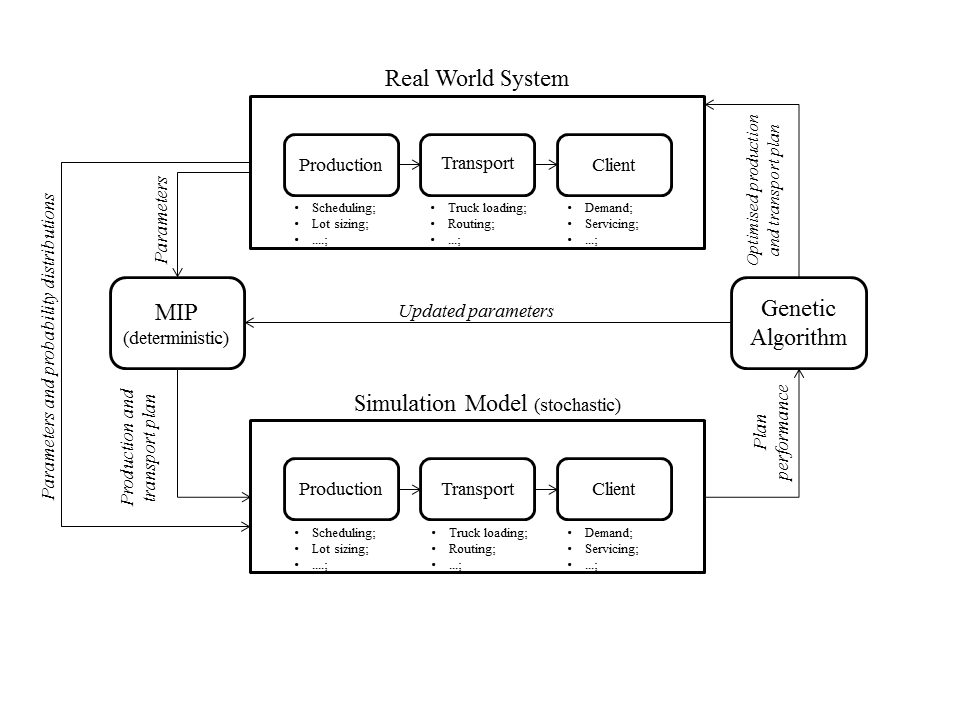
\includegraphics[width=.6\linewidth]{C:/ProjetosGithub/Monografia/Imagens/intro001.png}
\caption*{Fonte: Frazzon et al. (2017)}
\label{fig:intro001}
\end{figure}

O ganho computacional proveniente do uso de uma estratégia mais leve pode dar base para uma extensão dos modelos de planejamento integrado, tendo em vista que hoje inexiste um modelo de planejamento integrado que envolva tanto o planejamento do estoque de matéria prima quanto os planejamentos de produção e transportes.

O presente projeto de pesquisa tem como objetivo comparar diferentes modelos de otimização para o problema de controle integrado de estoques de matéria prima, programação da produção e programação de transportes.

\hypertarget{objetivos}{%
\section{OBJETIVOS}\label{objetivos}}

\hypertarget{objetivo-geral}{%
\subsection{Objetivo geral}\label{objetivo-geral}}

O objetivo da presente trabalho é de comparar diferentes cenários de otimização para uma cadeia de suprimentos a fim de mensurar qual o melhor modelo proposto.

\hypertarget{objetivos-especuxedficos}{%
\subsection{Objetivos específicos}\label{objetivos-especuxedficos}}

\begin{enumerate}
\def\labelenumi{\arabic{enumi}.}
\tightlist
\item
  Realizar revisão bibliométrica e de conteúdo sobre os tópicos envolvidos;
\item
  Revisar principais métodos / tecnologias de planejamento integrado;
\item
  Comparar os resultados dos modelos já validados na literatura;
\item
  Avaliar o desempenho dos modelos utilizando dados provenientes de uma potencial aplicação real, analisando potenciais ganhos em termos de desempenho operacional em cenários envolvendo comportamentos estocásticos.
\end{enumerate}

\hypertarget{delimitauxe7uxf5es-do-trabalho}{%
\section{DELIMITAÇÕES DO TRABALHO}\label{delimitauxe7uxf5es-do-trabalho}}

A implementação se limitará a considerar estoque de matéria-prima, produção e transporte. Áreas adjacentes podem estar presentes na simulação, mas não serão consideradas nas variáveis de decisão.

\hypertarget{estrutura-do-trabalho}{%
\section{ESTRUTURA DO TRABALHO}\label{estrutura-do-trabalho}}

Em desenvolvimento.

\hypertarget{revisuxe3o-da-literatura}{%
\chapter{REVISÃO DA LITERATURA}\label{revisuxe3o-da-literatura}}

Ao longo dos anos, prevaleceu a visão de uma empresa que trabalha não isolada, mas em conjunto com outras empresas (Chae et al., 2014). Assim, estruturas da cadeia de suprimentos cada vez mais complexas em ambientes dinâmicos exigem capacidade de resposta e produtividade, nas quais os recursos existentes do sistema são empregados da maneira mais eficiente possível (Ehm et al., 2015; Frazzon, Albrecht, et al., 2018). A indústria 4.0 e sua ampla gama de conceitos e tecnologias (Lasi et al., 2014) podem contribuir para a materialização da produtividade e da capacidade de resposta. No entanto, conectar muitas organizações, operações e clientes leva a um cenário de alta incerteza de diferentes fontes (Peidro et al., 2009). No entanto, isso deve ser considerado nas questões de planejamento e controle, a fim de obter políticas e planos robustos.

Para lidar com esse comportamento, a otimização baseada em simulação é uma abordagem que possui recursos para lidar eficientemente com um cenário estendido, levando em consideração a dinâmica dos sistemas, levando a soluções quase ótimas em um tempo viável (Liotta et al., 2016). Métodos baseados em simulação podem ser usados para desenvolver e avaliar sistemas complexos. Aspectos como configuração física ou regras operacionais de um sistema podem ser considerados. Suas aplicações cresceram em diversas áreas, auxiliando os gerentes no processo de tomada de decisão e permitindo uma melhor compreensão dos processos em sistemas complexos (Sakurada e Miyake, 2009). Essas premissas são expressas em relações matemáticas, lógicas e simbólicas entre as entidades ou objetos de interesse do sistema. Dessa forma, as possíveis alterações do sistema podem primeiro ser simuladas para prever seu impacto no desempenho do sistema. Além disso, a simulação também permite ao tomador de decisão avaliar várias políticas de controle (Pirard et al., 2011). Numerosas réplicas das simulações podem ser realizadas para avaliar a robustez do projeto implementado. Infelizmente, a simulação não garante um design ideal. No entanto, a desvantagem apresentada pode ser equilibrada com a integração de outras ferramentas, como a modelagem matemática.

A combinação de modelos de simulação e programação matemática em um esquema iterativo, visa avaliar os efeitos das decisões no desempenho de um sistema de manufatura. Assim, trabalhos nesse sentido concentram-se na integração de diferentes metodologias de modelagem, a fim de combinar as vantagens oferecidas por cada uma delas na solução de problemas complexos. Os modelos analíticos buscam soluções que avaliam os valores ideais das variáveis de decisão. No entanto, as soluções fornecidas são geralmente limitadas em seus campos de aplicação devido a premissas restritivas predeterminadas. Os modelos de simulação, por sua vez, são mais capazes de capturar o comportamento real do sistema, mas não são adequados para resolver problemas de otimização. A integração de modelos analíticos e de simulação, também chamados de modelos híbridos, leva a representar uma opção promissora para melhores resultados (Lin e Chen, 2015). Assim, os modelos híbridos buscam combinar as vantagens e evitar as desvantagens de ambas as ferramentas (Peidro et al., 2009).

\hypertarget{metodologia}{%
\chapter{METODOLOGIA}\label{metodologia}}

A metodologia a ser aplicada será de simulação.

Esse capítulo será melhor desenvolvido quando for terminada a revisão de literatura.

\hypertarget{resultados-e-discussuxf5es}{%
\chapter{RESULTADOS E DISCUSSÕES}\label{resultados-e-discussuxf5es}}

Working on it :)

\hypertarget{conclusuxe3o}{%
\chapter{CONCLUSÃO}\label{conclusuxe3o}}

Working on it :)

\hypertarget{referuxeancias-bibliogruxe1ficas}{%
\chapter*{REFERÊNCIAS BIBLIOGRÁFICAS}\label{referuxeancias-bibliogruxe1ficas}}
\addcontentsline{toc}{chapter}{REFERÊNCIAS BIBLIOGRÁFICAS}

Arica, E., \& Powell, D. J. (2014). A framework for ICT-enabled real-time production planning and control. Advances in Manufacturing, 2(2), 158--164. \url{http://doi.org/10.1007/s40436-014-0070-5}

Banks, J. (1998). Handbook of simulation: principles, methodology, advances, applications, and practice. John Wiley \& Sons.

Banks, J., Carson, J., Nelson, B., \& Nicol, D. (2000). Discrete-Event System Simulation. Englewood Cliffs, NJ, USA: Prentice Hall.

Chen, Z. (2004). Integrated Production and Distribution Operations: Taxonomy, Models, and Review. Handbook of Quantitative Supply Chain Analysis Modeling in the EBusiness Era, 1--32. \url{http://doi.org/10.1007/978-1-4020-7953-5_17}

Chen, Z.-L., \& Vairaktarakis, G. L. (2005). Integrated Scheduling of Production and Distribution Operations. Management Science, 51(4), 614--628. \url{http://doi.org/10.1287/mnsc.1040.0325}

Christopher, M. (2005). Logistics and supply chain management: creating value-added networks. Pearson Education.

Devapriya, P., Ferrell, W., \& Geismar, N. (2016). Integrated Production and Distribution Scheduling with a Perishable Product. European Journal of Operational Research, 259, 906--916. \url{http://doi.org/10.1016/j.ejor.2016.09.019}

Frazzon, E. M., Albrecht, A., Pires, M., Israel, E., Kück, M., \& Freitag, M. (2017). Hybrid approach for the integrated scheduling of production and transport processes along supply chains. International Journal of Production Research, 7543(July), 0. \url{http://doi.org/10.1080/00207543.2017.1355118}

Ivanov, D. (2010). An adaptive framework for aligning (re)planning decisions on supply chain strategy, design, tactics, and operations. International Journal of Production Research, 48(13), 3999--4017. \url{http://doi.org/10.1080/00207540902893417}

Lee, J., Bagheri, B., \& Kao, H. A. (2015). A Cyber-Physical Systems architecture for Industry 4.0-based manufacturing systems. Manufacturing Letters, 3, 18--23. \url{http://doi.org/10.1016/j.mfglet.2014.12.001}

Lin, J. T., \& Chen, C.-M. (2015). Simulation optimization approach for hybrid flow shop scheduling problem in semiconductor back-end manufacturing. Simulation Modelling Practice and Theory, 51, 100--114. \url{http://doi.org/10.1016/j.simpat.2014.10.008}

Monostori, L., Kádár, B., Bauernhansl, T., Kondoh, S., Kumara, S., Reinhart, G., \ldots{} Ueda, K. (2016). Cyber-physical systems in manufacturing. CIRP Annals - Manufacturing Technology. \url{http://doi.org/10.1016/j.cirp.2016.06.005}

Mula, J., Peidro, D., Díaz-Madroñero, M., \& Vicens, E. (2010). Mathematical programming models for supply chain production and transport planning. European Journal of Operational Research, 204(3), 377--390. \url{http://doi.org/10.1016/j.ejor.2009.09.008}

Narasimhan, R., \& Mahapatra, S. (2004). Decision models in global supply chain management. Industrial Marketing Management, 33(1), 21--27. \url{http://doi.org/10.1016/j.indmarman.2003.08.006}

O'Kane, J. F., Spenceley, J. R., \& Taylor, R. (2000). Simulation as an essential tool for advanced manufacturing technology problems. Journal of Materials Processing Technology, 107(1--3), 412--424. \url{http://doi.org/10.1016/S0924-0136(00)00689-0}

Pirard, F., Iassinovski, S., \& Riane, F. (2011). A simulation based approach for supply network control. International Journal of Production Research, 49(24), 7205--7226. \url{http://doi.org/10.1080/00207543.2010.518726}

Sakurada, N., \& Miyake, D. I. (2009). Aplicação de simuladores de eventos discretos no processo de modelagem de sistemas de operações de serviços. Gestão \& Produção, 16(1), 25--43. \url{http://doi.org/10.1590/S0104-530X2009000100004}

Scholz-Reiter, B., Makuschewitz, T., Novaes, A. G. N. N., Frazzon, E. M., Jr., O. F. L., \& Lima, O. F. (2011). An approach for the sustainable integration of production and transportation scheduling. International Journal of Logistics Systems and Management, 10(2), 158. \url{http://doi.org/10.1504/IJLSM.2011.042626}

  \bibliography{book.bib}

\end{document}
